\setlength\intextsep{1mm}

\section*{\textbf{Task 1: Comparing standard normalization to PCA-sphering on MNIST}}

%	Task 1:
%	1. You should return 5 plots: 1 for each cost individually, 1 with all the costs together, 1 with all the accuracies. 
%	    Plot of the cost functions over the 10 runs
%	    Plot of the accuracies over the 10 runs
%	2. choice of gamma for:
%	    Raw data without normalization 
%	    Standard normalized data
%	    PCA-sphered data
%	3. An explanation of what you see

\textbf{1.} Cost history plots during training of using \textbf{original data}, \textbf{standard normalized data}, and \textbf{PCA-spehered data}.

\begin{figure}[H]
    \centering
    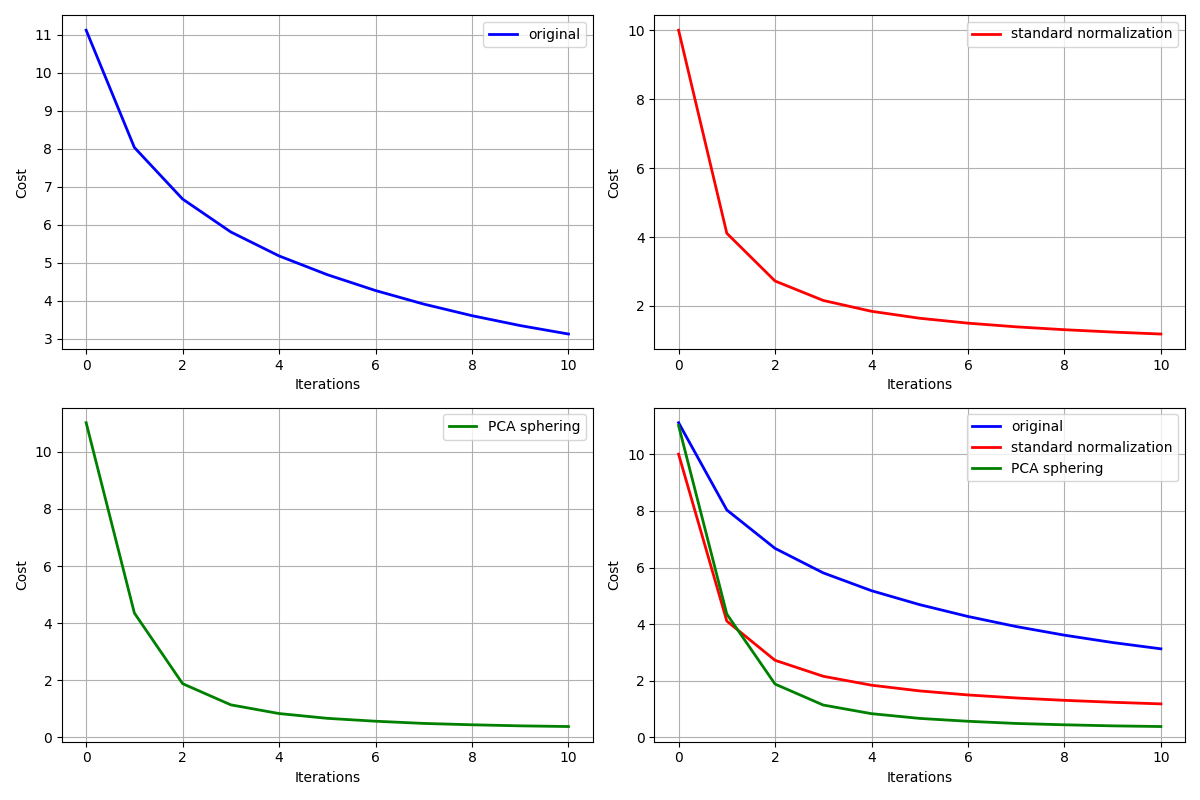
\includegraphics[width=120mm]{task1-cost.png}
    \caption{Cost history plots (individually and all together) over 10 iterations}
    \label{fig:task1}
\end{figure}


\textbf{2.} Plot of the accuracies over the 10 iterations
\begin{figure}[H]
    \centering
    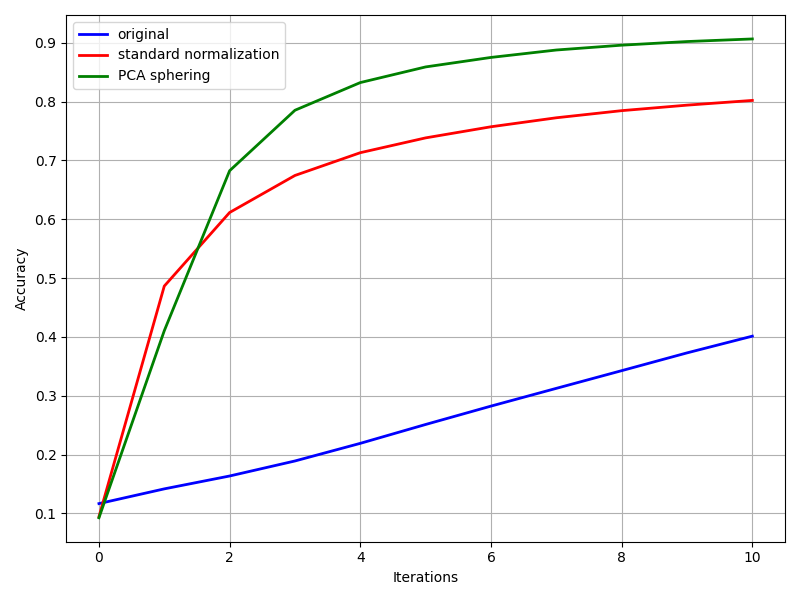
\includegraphics[width=80mm]{task1-accuracy.png}
    \caption{Accuracy over 10 iterations}
    \label{fig:task2}
\end{figure}

\textbf{3.} Choice of gamma (the exponent of learning rate $\alpha$) for \textbf{original data}, \textbf{standard normalized data}, and \textbf{PCA-spehered data}

\begin{table}[H]
    \centering
    \begin{tabular}{|c|c|}
    \hline
         Data &  gamma  \\
        \hline
         original data & -5 \\
         standard normalized data & 0   \\
         PCA-spehered data & 1   \\
        \hline
    \end{tabular}
    \caption{gamma values during training}
    \label{tab:gamma}
\end{table}

\textbf{4.} Explanation of what I see \\
After applying ten iterations of trainings using data engineered differently, clearly traing using the PCA-sphered data produced the lowest cost and also the highest accuracy. This means PCA-sphered data is the most benefical feature engineering method in the given multiclass classification problem.




\newpage
\section*{\textbf{Task 2: Exploring predictors of housing prices }}
% 1. Histogram of weights for:
%   lambda = 0
%   lambda = 50
%   lambda = 100
%   lambda = 150
% 2. Step length, number of steps, and final cost for the figures
% 3. Plot the cost history for each lambda to demonstrate that your model converged. 
% 4. Explanation of what you see (and whether or not you can recreate the plots)



\textbf{1.} Histogram of weights for $\lambda$ = 0, 50, 100, 150.

\begin{figure}[H]
    \centering
    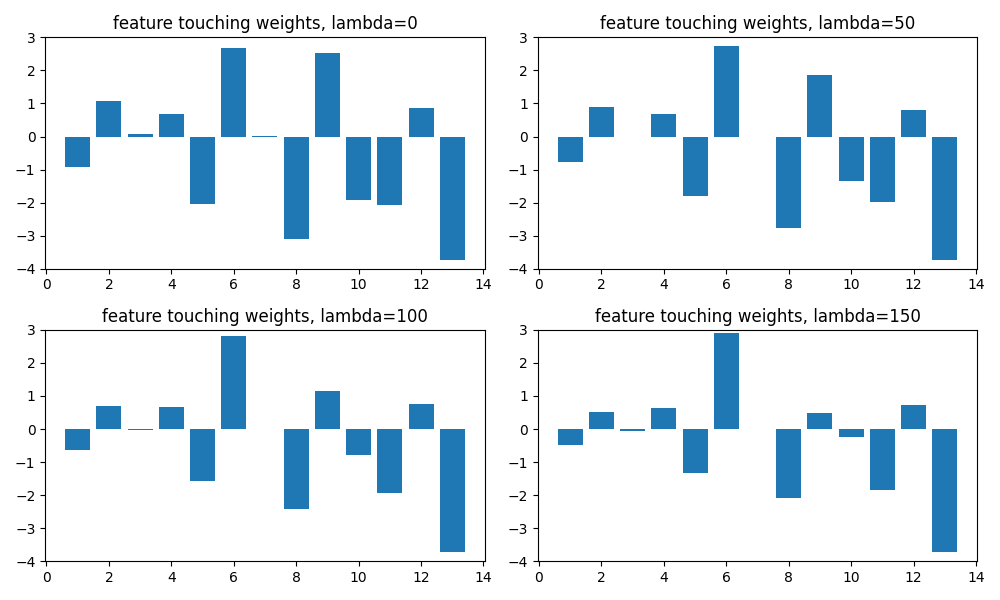
\includegraphics[width=120mm]{task2-weights.png}
    \caption{Feature-touching weights for trainings of using different $\lambda$}
    \label{fig:task2-weights}
\end{figure}


\textbf{2.} Step length, number of steps, and final cost.
\begin{table}[H]
    \centering
    \begin{tabular}{|c|c|c|c|}
        \hline
         $\lambda$ &  step length &  number of steps (iterations) & final cost \\
        \hline
         0 & 0.1 & 400 & 22.778 \\
         50  & 0.1 & 400 & 25.066 \\
         100  & 0.1 & 400 & 26.652 \\
         150 & 0.1 & 400 & 28.176 \\
        \hline
    \end{tabular}
    \caption{Hyperparameters}
    \label{tab:hyperparams}
\end{table}

\textbf{3.} Cost history plots.

\begin{figure}[H]
    \centering
    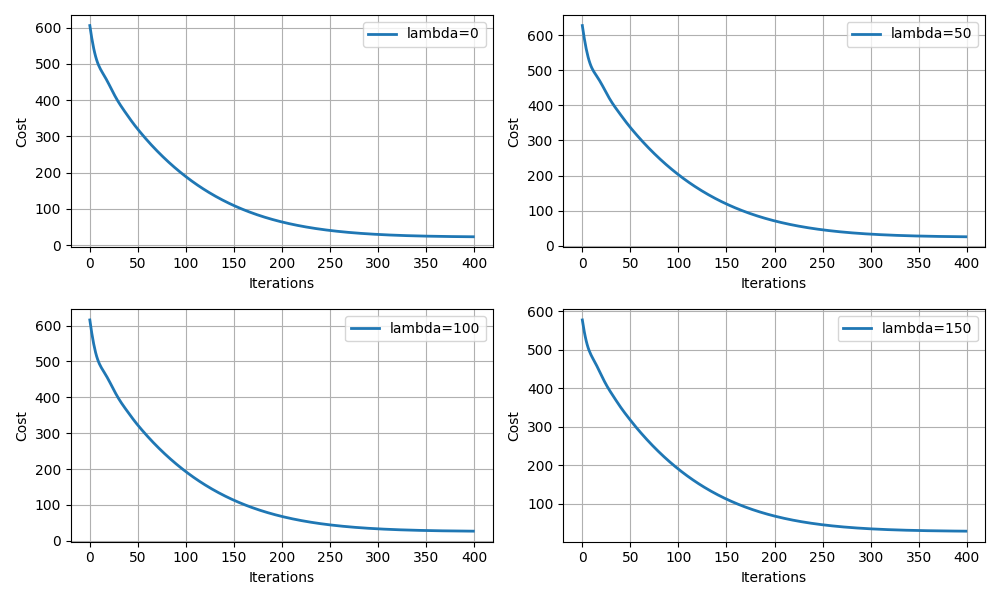
\includegraphics[width=120mm]{task2-costs.png}
    \caption{Cost history for each $\lambda$}
    \label{fig:task2-cost}
\end{figure}

\textbf{4.} Explanation of what I see \\
Based on Figure 3, there are some weights whose "bars" (absoulte values) are consistently large, such as w6, w8, w13, meaning that they corresponds to the most important features. However, some weights are diminishing as $\lambda$ increases, such as w5, w9, w10, meaning that the corresponding features are relatively unimportant.

